\documentclass{article}

\usepackage{arxiv}
\usepackage{amsmath, amsfonts, amssymb}
\usepackage{graphicx}
\usepackage{hyperref}
\usepackage{booktabs}
\usepackage{float}
\usepackage{tikz}
\usetikzlibrary{arrows.meta, positioning, shapes.geometric, calc}
\setlength{\headheight}{23pt}
\makeatletter
\def\headeright{}
\def\undertitle{}
\makeatother
\AtBeginDocument{
  \setlength{\headheight}{23pt}
  \addtolength{\topmargin}{-9pt}
}

\title{Shared Execution Graphs:\\
A Substrate for Multi-Agent and Human-AI Collaboration}

\author{
  Josh Rosen \\
  ThruWire, Inc.
  \And
  Seth Rosen \\
  ThruWire, Inc.
}

\begin{document}

\maketitle

\begin{abstract}
In many multi-agent and human-AI systems, each participant is incentivized to be locally heroic: solve the task in front of it, emit a plausible answer, and move on. That behavior can be effective for a single step, but it scales poorly when many humans and agents share evolving state. Intermediate artifacts, assumptions, and downstream dependencies drift apart because each actor optimizes for local task completion rather than stewardship of the whole computational process. The result is collaborative state that may look productive in transcripts while becoming structurally incoherent under revision.

This paper argues that collaboration for AI-native work should be grounded in a shared execution graph rather than isolated chat loops or shared memory alone. A shared execution graph is a durable directed acyclic graph of blocks, tasks, or notebooks with explicit dependencies, replayable execution identities, inspectable intermediate artifacts, and incremental recomputation semantics. It is shared because multiple humans, agents, and tools can read, edit, execute, review, and consume the same graph state. In this model, collaboration is not merely communication about work. It is joint stewardship of a shared computational structure.

We build on prior work on execution lineage and artifact-centric state, but the present paper is self-contained and asks a different systems question: how should multiple participants coordinate over executable shared state? We distinguish shared execution from shared memory, compare graph-based collaboration to chat rooms, shared documents, wikis, git repositories, task queues, knowledge graphs, vector memory, blackboard systems, and message-passing multi-agent loops, and argue that these alternatives usually lack the dependency-aware propagation semantics required for maintained collaborative state.

The contribution is a systems-level abstraction, not a claim that shared graphs eliminate conflict or replace all collaboration interfaces. Graph authoring has overhead, many tasks remain well served by lightweight conversation, and conflict resolution still requires policy and sometimes human judgment. The narrower claim is that for long-lived AI-native work, a shared execution graph is a stronger collaboration substrate than shared chat, shared memory, or shared documents because it preserves explicit dependency structure, execution identity, and consistent propagation under change.
\end{abstract}

\section{Introduction}

Human-AI collaboration is often described as conversation. A user asks, the model answers, follow-up questions accumulate, and the thread grows into a working session. Multi-agent systems generalize the same pattern: one agent plans, another researches, another critiques, and coordination happens through message passing, role prompts, shared notes, or a memory store \cite{yao2023react,li2023camel,wu2023autogen,hong2023metagpt}. This pattern is productive because it matches the interface of current language models. The simplest control loop is also the default interface.

That interface, however, becomes structurally weak once work is long-lived. Many real tasks are not single conversational episodes. They produce intermediate analyses, assumptions, plans, decision artifacts, transformations, and revisions that must remain coherent across repeated edits by multiple humans and multiple agents. In these settings, the system's main challenge is no longer only answer generation. It is maintaining shared state under change.

One reason current collaboration degrades is behavioral as much as representational: each actor tends to optimize for solving its own visible subtask. An agent asked for a plan tries to finish the plan. A reviewer asked for comments tries to finish the review. A research agent tries to add findings quickly. Each can succeed locally while leaving the shared system globally inconsistent. Once many actors operate in parallel, this ``be the hero'' pattern becomes a scaling failure because no one is explicitly responsible for preserving coherent dependencies, artifact authority, invalidation state, or downstream correctness.

Prior work on execution lineage and artifact-centric state makes a stronger alternative available. If AI-native work executes through explicit graphs and publishes durable intermediate artifacts, then collaboration can be organized around maintaining that executable state rather than around passing messages about it. That leads to the central question of this paper:
\begin{quote}
If AI-native work executes as a graph and produces durable artifact state, how should multiple humans and agents collaborate over that state?
\end{quote}

The common answer today is some mixture of messaging and auxiliary stores. Agents talk to each other. Humans leave instructions in chats, documents, tickets, wikis, or pull requests. Systems maintain long-term memory in vector stores or knowledge bases. These mechanisms are useful, but they usually coordinate \emph{around} the work rather than \emph{through} the work. They preserve facts, notes, messages, or outputs, yet they often do not preserve which exact execution produced an artifact, which downstream artifacts depend on it, whether an upstream change invalidates that artifact, or what must be recomputed next.

This distinction motivates the paper's core claim:
\begin{quote}
Collaboration is not merely communication; it is stewardship of a shared computational structure.
\end{quote}

We call that structure a \emph{shared execution graph}. It is a directed acyclic graph (DAG) of blocks, notebooks, or tasks with explicit dependency edges, replayable execution identities, typed intermediate artifacts, and propagation semantics. It is shared because all participants---humans, autonomous agents, code assistants, tools, and external services---can inspect and mutate the same substrate. Messages may still exist, but they are no longer the authoritative state boundary. The graph is.

This shift matters because \emph{shared memory is not the same as shared execution}. A memory store may tell an agent that a recommendation changed. A shared execution graph tells the system which block changed, which artifact it superseded, which downstream blocks now have stale reads, which branches remain unaffected, and which recomputations or reviews should follow. The first is a coordination hint; the second is a collaboration substrate.

The paper makes four contributions. First, it defines the shared execution graph as a collaboration substrate that turns shared work into an explicit object of stewardship rather than a side effect of message exchange. Second, it formalizes actors, mutations, execution identity, and propagation semantics for multi-human and multi-agent work. Third, it introduces a concurrency and conflict model centered on graph mutation, stale state detection, invalidation, attribution, and reviewable edits rather than on informal message coordination alone. Fourth, it proposes an evaluation framework in which collaborative systems are judged not only by final output quality, but also by maintained collaborative state quality over time.

The scope is intentionally restrained. We do not claim that all collaboration should become graph-native, that conversation is obsolete, or that shared graphs remove disagreement. Many tasks do not justify graph authoring overhead. Some collaborative ambiguity is irreducibly social. Agents can also make poor structural edits, and poorly designed dependency semantics can create false confidence. The narrower thesis is that when work is multi-step, multi-actor, revisable, and execution-dependent, a shared execution graph is a materially stronger substrate than shared chat transcripts, message loops, or generic memory stores.

\section{Motivating Example}

Consider a strategy workflow shared by two humans and three agents. A human researcher authors an upstream market-structure block. A research agent expands the graph with competitor profiles and customer segmentation artifacts. A planning agent consumes those artifacts to draft rollout options. A finance-minded human edits an upstream assumptions block to require that year-one launch remain budget-neutral. A review agent checks whether the downstream strategy memo and implementation plan still conform.

In a loop-centric system, this work commonly fragments. The human researcher has one chat. The planning agent has another. The review agent reads a shared document plus a few notes in a wiki or ticket system. The updated budget constraint may be mentioned in a message, copied into a planning brief, and partially reflected in a revised memo. But there is no authoritative computational object that knows exactly which downstream artifacts depend on the changed assumption. One agent may continue using the old segmentation summary. Another may rewrite the final memo correctly while leaving the rollout plan stale. Each actor looks productive within its local loop, yet the collaboration as a whole accumulates state debt because nobody is operating as steward of the shared computational state.

Now contrast a shared execution graph. The market assumptions, competitor profiles, segmentation, rollout criteria, implementation plan, and final memo are explicit blocks with explicit dependencies. The budget-neutrality change is a graph mutation against a concrete upstream block or artifact. The runtime can mark downstream artifacts as stale, preserve unrelated branches exactly, and schedule recomputation or review where appropriate. Humans and agents can both inspect the affected subgraph before choosing whether to recompute automatically, request approval, or manually edit a downstream node. The graph therefore changes the expected behavior of each participant: instead of merely solving a local task, each actor must reason about affectedness, publication authority, and the coherence of the maintained whole.

The difference is not merely better storage. Both systems may preserve the same text somewhere. The difference is that one preserves \emph{execution structure}. In the graph case, participants share the same object of collaboration: a dependency-aware, executable, replayable structure. In the loop case, collaboration is mediated by communication plus reconstruction.

Figure~\ref{fig:collaboration-contrast} illustrates the contrast. On the left, state fragments across chats, documents, and memory stores, with downstream impact inferred socially or heuristically. On the right, humans, agents, and tools all operate on a shared execution graph whose explicit dependencies support invalidation and propagation.

\begin{figure}[t]
\centering
\begin{tikzpicture}[
  font=\small,
  scale=0.82,
  transform shape,
  actor/.style={draw, rounded corners, align=center, minimum width=18mm, minimum height=7mm, fill=black!3},
  store/.style={draw, rounded corners, align=center, minimum width=20mm, minimum height=7mm, fill=black!6},
  block/.style={draw, rounded corners, align=center, minimum width=19mm, minimum height=7mm, fill=black!4},
  note/.style={draw, rounded corners, align=left, minimum width=28mm, minimum height=8mm, fill=black!2},
  arr/.style={-{Stealth[length=2mm]}, thick},
  dasharr/.style={-{Stealth[length=2mm]}, dashed, thick}
]
\node[font=\bfseries] at (0,0.3) {Fragmented loop-centric collaboration};
\node[actor] (h1) at (-2.7,-0.8) {Human A};
\node[actor] (a1) at (0,-0.8) {Agent 1};
\node[actor] (a2) at (2.7,-0.8) {Agent 2};
\node[store] (chat1) at (-3.0,-2.1) {chat};
\node[store] (doc1) at (-0.7,-2.1) {doc};
\node[store] (mem1) at (1.6,-2.1) {memory};
\node[store] (wiki1) at (3.7,-2.1) {wiki};
\node[note] (frag) at (0.5,-4.0) {state is shared indirectly\\through messages and notes\\dependency impact is inferred};
\draw[arr] (h1) -- (chat1);
\draw[arr] (a1) -- (doc1);
\draw[arr] (a1) -- (mem1);
\draw[arr] (a2) -- (wiki1);
\draw[dasharr] (chat1) -- (doc1);
\draw[dasharr] (doc1) -- (mem1);
\draw[dasharr] (mem1) -- (wiki1);
\draw[dasharr] (frag.north) -- ($(doc1.south)!0.5!(mem1.south)$);

\node[font=\bfseries] at (10.6,0.3) {Shared execution graph collaboration};
\node[actor] (h2) at (7.2,-0.8) {Human};
\node[actor] (a3) at (10.6,-0.8) {Agent};
\node[actor] (t1) at (14.0,-0.8) {Tool};
\node[block] (b1) at (8.1,-2.2) {Assumptions};
\node[block] (b2) at (10.6,-2.2) {Research};
\node[block] (b3) at (13.1,-2.2) {Plan};
\node[block] (b4) at (10.6,-3.8) {Final memo};
\node[note] (prop) at (14.2,-4.2) {edit $\rightarrow$ affected subgraph\\$\rightarrow$ invalidation\\$\rightarrow$ recomputation / review};
\draw[arr] (h2) -- (b1);
\draw[arr] (a3) -- (b2);
\draw[arr] (t1) -- (b3);
\draw[arr] (b1) -- (b2);
\draw[arr] (b2) -- (b3);
\draw[arr] (b2) -- (b4);
\draw[arr] (b3) -- (b4);
\draw[dasharr] (h2.east) to[bend left=20] (b4.west);
\draw[dasharr] (a3.south) -- (b4.north);
\draw[dasharr] (prop.west) -- (b3.east);
\end{tikzpicture}
\caption{Messages and shared memory can coordinate participants, but they usually lack explicit execution and propagation semantics. A shared execution graph gives humans, agents, and tools one authoritative substrate for edits, replay, invalidation, and recomputation.}
\label{fig:collaboration-contrast}
\end{figure}

\section{Background and Related Work}

\subsection{Agent Loops and Multi-Agent Coordination}

ReAct \cite{yao2023react} made the reasoning-and-acting loop the canonical LLM-agent pattern. Toolformer \cite{schick2023toolformer} showed how tool use can be integrated into model behavior. Multi-agent systems such as CAMEL \cite{li2023camel}, AutoGen \cite{wu2023autogen}, MetaGPT \cite{hong2023metagpt}, and Voyager \cite{wang2023voyager} extend this idea through role specialization, conversation protocols, and iterative critique. These systems demonstrate that complex tasks can be decomposed across interacting agents even when the dominant coordination primitive remains messaging.

The important limitation for our purposes is not that message passing fails. It often works. The limitation is that coordination state is commonly encoded in transcripts, agent-local memory, or controller logic rather than in a shared execution substrate. Even when several agents work on one task, their notion of ``current state'' often depends on prompt reconstruction rather than on a common dependency-aware object.

\subsection{Execution Lineage and Artifact-Centric State}

Prior work on execution lineage argues that AI-native work benefits from explicit DAG structure with replayable execution identities, deterministic forward execution, and selective recomputation boundaries. Related work on artifact-centric state argues that such execution requires durable intermediate artifacts with lineage, addressability, and supersession semantics. The present paper builds on those abstractions directly. A shared execution graph is therefore not merely a task graph. It is an execution-lineage graph whose nodes publish artifact-centric state.

This framing is adjacent to recent work on agent harnesses and workflow memory \cite{pan2026nlah,zhang2025harness,wang2024awm,fan2024workflowllm,han2025legomem,yan2025memoryr1,borro2026memori}. Harness research recognizes that important behavior lives outside the raw model invocation. Memory research recognizes that long-lived agents require durable external state. Our claim is narrower and more structural: memory helps an actor remember; a shared execution graph defines the collaboration substrate over which actors coordinate, mutate, and propagate work.

\subsection{Workflow DAGs, Provenance, and Replay}

Workflow systems such as Dryad \cite{isard2007dryad}, Spark \cite{zaharia2016spark}, Airflow \cite{airflowdocs}, and dbt \cite{dbtdocs} long ago converged on explicit dependency graphs, materialized intermediates, and lineage-aware recomputation. Provenance research similarly studies how outputs can be traced to prior state \cite{buneman2001why,freire2008provenance}. The relevance is not metaphorical. These systems show that when work becomes multi-stage and collaborative, implicit dependencies and ad hoc handoffs become bottlenecks for correctness and maintainability.

LLM workflows differ because node-local computation may be stochastic and semantically rich. But the need for explicit dependency semantics becomes stronger, not weaker, when collaboration involves revisable intermediate reasoning rather than only deterministic transforms.

\subsection{Blackboard Systems, Shared Memory, and Collaborative Editing}

Blackboard architectures are a historically important comparison because they also provide a shared space where multiple knowledge sources contribute partial work. Nii's classic blackboard formulation emphasized a common store visible to specialist modules \cite{nii1986blackboard}. That tradition correctly recognized that shared intermediate state can outperform isolated agent behavior. Our distinction is that a generic blackboard usually does not by itself define replayable execution identity, explicit downstream invalidation semantics, or graph-scoped recomputation boundaries for AI-native work. A shared execution graph can be seen as a more execution-precise substrate built around lineage and dependency structure rather than only shared posting.

Collaborative editing research, including operational transformation and CRDTs \cite{ellis1989groupware,shapiro2011crdt}, is also relevant because it studies how concurrent edits can remain intelligible and mergeable. We do not claim that graph collaboration reduces to text-collaboration algorithms. The point is more limited: shared execution graphs inherit the need for explicit concurrency semantics, stale-read handling, attribution, and conflict visibility. Those questions are familiar in CSCW and distributed systems even if the objects being edited are now executable blocks and artifacts rather than plain documents.

\subsection{Human-AI Collaboration}

Human-AI interaction research has increasingly emphasized oversight, review, trust, and interface structure rather than pure model accuracy \cite{amershi2019guidelines}. That perspective aligns with our evaluation stance. The relevant system quality is not only whether the model can produce a good answer once, but whether humans can understand what changed, what remains stale, what needs review, and how the system is maintaining shared state over time.

\section{Problem Formulation}

We consider AI-native work that is collaborative along at least one of three axes:
\begin{itemize}
\item multiple humans contribute edits, review, or decisions
\item multiple agents produce, transform, or critique intermediate work
\item work persists across time and must be revised under changing assumptions
\end{itemize}

The dominant loop-centric approach typically treats each actor as owning a local context window and coordinating through messages or externalized notes. This creates a predictable behavioral bias: each actor is rewarded for solving the local subproblem it can see, not for maintaining the global integrity of the shared system. Let $A = \{a_1, \dots, a_n\}$ be actors, each with local state $L_i$, and let coordination occur through messages $M$ plus an auxiliary shared store $S$:
\begin{equation}
\text{collaboration}_{\mathrm{loop}} = \{L_i\}_{i=1}^{n} + M + S
\end{equation}

This arrangement can preserve a large amount of information, but it leaves four recurrent problems under-specified.

\paragraph{Execution identity is weak.}
When an output is revised, the system often cannot say which exact prior execution it corresponds to, whether it is a replay of prior work, or whether it is merely a fresh generation that resembles earlier content.

\paragraph{Dependency structure is weak.}
Messages and documents may mention upstream relationships, but they usually do not make those relationships operational. The system often does not know which downstream work is affected when upstream reasoning changes.

\paragraph{Propagation is heuristic.}
If an upstream assumption changes, propagation is commonly manual, prompt-assembled, or partial. Systems may rewrite the final answer while leaving stale intermediates elsewhere.

\paragraph{Conflict visibility is weak.}
Two actors can make incompatible edits against overlapping state without the system surfacing that incompatibility until late human review, because the authoritative collaboration object is ambiguous.

These failures are all variants of the same structural issue: \emph{shared state is not the same as shared execution}. A wiki page, vector store, or task queue can preserve shared information while remaining silent about which computations that information should invalidate or regenerate. They also leave the burden of systems thinking implicit. Each participant must infer whether it is safe to proceed, what else is affected, and whether its local success will create downstream incoherence.

We therefore define the target object differently. Let
\begin{equation}
G = (V, E)
\end{equation}
be a directed acyclic graph of executable blocks or tasks, where each node $v \in V$ publishes artifacts and each edge $(u,v)\in E$ is an explicit dependency relation. We want collaboration to occur through mutations of $G$ and of its artifact state, not only through messages about $G$.

The systems question is then:
\begin{quote}
What collaboration semantics are gained when humans, agents, and tools share one executable dependency graph with stable execution identities and propagation rules?
\end{quote}

\section{Shared Execution Graph Model}

\subsection{Definition}

A \emph{shared execution graph} is a tuple
\begin{equation}
\mathcal{C} = (G, X, R, \Pi)
\end{equation}
where:
\begin{itemize}
\item $G=(V,E)$ is an executable DAG of blocks or tasks
\item $X$ is the current set of published artifacts and execution records
\item $R$ is the set of actors authorized to inspect, mutate, execute, or review parts of the graph
\item $\Pi$ is the policy layer governing invalidation, recomputation, approval, and conflict handling
\end{itemize}

Each node $v$ has a structural specification $\sigma_v$, a resolved input surface $x_v$, a local execution procedure $f_v$, and a published output boundary $o_v$. Following the execution-lineage formulation, we define execution identity as:
\begin{equation}
k_v = h(\sigma_v, x_v, \{k_u : u \in \mathrm{pred}(v)\})
\end{equation}
where $\mathrm{pred}(v)$ are the immediate predecessors of $v$. Following the artifact-centric formulation, the published result of a node is not just text but a durable artifact surface with lineage and status.

The collaboration-specific extension is that multiple actors may inspect or mutate $\sigma_v$, $x_v$, dependency edges, publication metadata, or review status over time. Those edits operate against explicit graph structure rather than only against informal narrative context.

\subsection{Why Shared Execution Is Stronger Than Shared Memory}

A shared memory system provides a common place to read and write information. A shared execution graph provides a common place to read and write \emph{dependency-bearing computational state}. The difference matters in three ways.

\paragraph{Identity.}
Graph nodes and published artifacts have identities grounded in executions and dependencies, not only in document names or memory keys.

\paragraph{Affectedness.}
The graph can enumerate affected downstream work after an edit. A generic shared memory store usually cannot do this without an added dependency model.

\paragraph{Propagation.}
The graph can invalidate, replay, or recompute downstream work consistently. A shared memory store may preserve the changed fact but not the semantics of what to do next.

This distinction is the collaboration analogue of the earlier distinction between prompt lineage and execution lineage. Shared memory preserves recall; shared execution preserves coordinated maintenance.

\subsection{Graph Mutations as Collaboration Units}

In loop-centric collaboration, the primitive unit is often the message: ``please update the memo,'' ``agent 2 found a new source,'' or ``assume budget neutrality.'' In shared execution collaboration, the stronger primitive is the graph mutation. A mutation can:
\begin{itemize}
\item add a node or dependency edge
\item edit a node specification or prompt contract
\item supersede an artifact
\item trigger invalidation or recomputation
\item mark a node for review, repair, or approval
\end{itemize}

Messages can still accompany these operations, but the authoritative state change is the mutation against the graph or its published artifacts. This makes collaboration semantics stronger than conversational intent alone.

\section{Actors, Mutations, and Execution Identity}

\subsection{Actors}

We distinguish four broad actor classes.

\paragraph{Humans.}
Humans may author structure, edit assumptions, inspect intermediate artifacts, approve or reject changes, resolve conflicts, and interpret ambiguous goals.

\paragraph{Autonomous agents.}
Agents may propose new nodes, execute existing nodes, critique downstream outputs, monitor stale regions, repair failed nodes, or synthesize summaries over graph state.

\paragraph{External tools and services.}
Tools may populate source artifacts, run validators, render outputs, execute code, or provide external data used by graph nodes.

\paragraph{Interactive clients.}
Chat clients, code assistants, or MCP-driven interfaces may present graph state conversationally while still reading from and writing to the graph as the authoritative backend.

The important point is that these actors can differ in interface while sharing the same substrate. One actor may experience the system as a visual DAG, another as a notebook-like builder, another as a chat interface with tool access. The collaboration model does not require one UI. It requires one authoritative execution graph and a shared obligation to preserve its coherence.

\subsection{Mutations}

Let a mutation be an operation $m$ that transforms collaboration state:
\begin{equation}
m : \mathcal{C}_t \rightarrow \mathcal{C}_{t+1}
\end{equation}
Examples include:
\begin{itemize}
\item editing upstream assumptions
\item adding a new analysis branch
\item changing a dependency edge
\item superseding an intermediate artifact
\item re-running a stale block
\item attaching a review decision to a recomputed node
\end{itemize}

Mutations matter because they are the place where collaboration becomes operational. A message saying ``budget neutrality now matters'' is not yet a maintained-state operation. A mutation that updates a criteria block or supersedes a recommendation artifact is. In that sense, a mutation is also a stewardship act: it changes the system's maintained state and therefore carries responsibility for affected downstream correctness.

\subsection{Execution Identity as Collaboration Grounding}

Execution identity provides the collaboration substrate with a concrete referent. Actors need not speak only about vague conversational state such as ``the analysis you did earlier.'' They can refer to a specific block execution or artifact version. This enables:
\begin{itemize}
\item exact replay rather than approximate regeneration
\item review of the precise state a downstream node consumed
\item auditability of who changed what and against which prior execution
\item reasoning about stale reads and recomputation scope
\end{itemize}

This is especially important in multi-agent work. Without execution identity, two agents can appear to operate on the ``same'' upstream note while actually consuming different prompt reconstructions or artifact versions. The graph eliminates some of this ambiguity by grounding collaboration in explicit execution records. That grounding is what lets actors reason meta-cognitively about the state they are inheriting rather than merely improvising from local context.

\subsection{Extending the Graph}

An important difference between graph-centric collaboration and question-answer chat is that agents can extend the graph itself. They are not limited to emitting free-form answers. An agent can add a competitor-analysis node, create a downstream risk review branch, or propose a repair block for inconsistent artifacts. Humans can approve these extensions, reject them, or rewire their dependencies.

This matters because collaborative AI work is often not just about filling in one output. It is about creating new structure as understanding evolves. A shared execution graph makes that structural growth inspectable and reviewable.

\section{Consistency, Invalidation, and Propagation}

\subsection{Consistency as a Graph Property}

In collaborative AI systems, consistency should not be framed only as agreement among messages. It should be framed as a property of the maintained graph state. A collaborative state is more coherent when:
\begin{itemize}
\item active artifacts agree with the current upstream assumptions they depend on
\item superseded artifacts are not mistaken for current ones
\item unaffected branches remain stable under irrelevant edits
\item affected downstream branches are identifiable and reviewable
\end{itemize}

Artifact-centric work describes maintained-state quality at the artifact level. Shared execution graphs generalize that concern to multiple actors maintaining a common dependency structure over time. This is the key behavioral shift: participants are evaluated not only on whether they contributed useful local work, but on whether their contributions preserve systemic coherence.

\subsection{Invalidation Before Recomputation}

An upstream edit should first create an invalidation judgment and only then a recomputation judgment. This sequencing matters. Without an explicit invalidation phase, downstream consumers can continue reading stale artifacts as if they were current while recomputation is pending or awaiting approval.

Formally, if node $u$ changes so that its execution identity becomes $k'_u \neq k_u$, then every reachable descendant $v$ whose identity function depends on $k_u$ becomes stale with respect to current state:
\begin{equation}
\mathrm{stale}(v) = 1 \quad \text{if} \quad k_v \text{ was computed from } k_u \text{ and } k'_u \neq k_u
\end{equation}
The system may then choose among replay, recomputation, manual review, or temporary suspension based on policy $\Pi$. But stale status should be visible before those downstream actions complete.

\subsection{Propagation Semantics}

Shared execution graphs support three useful propagation outcomes.

\paragraph{Exact preservation.}
If an edit occurs on an unrelated branch, unaffected downstream artifacts should remain exactly preserved. This is the no-op locality result already emphasized in prior execution-lineage evaluations.

\paragraph{Selective recomputation.}
If an upstream artifact changes in a dependency-relevant way, only affected descendants should be invalidated and recomputed.

\paragraph{Superseding publication.}
When recomputation produces a new current artifact, downstream consumers should see the superseding artifact as authoritative while historical versions remain available for audit.

These propagation semantics are stronger than what shared documents or chats normally provide. Those systems can record that something changed; they usually do not operationalize what the change should invalidate. A stewardship-oriented collaboration model requires exactly this operationalization because actors need the system to surface what responsible next action looks like.

\subsection{Inspectability}

Propagation is useful only if participants can inspect it. Humans and agents should be able to ask:
\begin{itemize}
\item what changed?
\item which upstream execution or artifact changed?
\item which downstream nodes are now stale?
\item which artifacts were preserved exactly?
\item which outputs were replayed, recomputed, or manually edited?
\end{itemize}

This is a major advantage over transcript-mediated collaboration. In a large chat or wiki-based workflow, these questions often require manual reconstruction from narrative history. The execution graph externalizes that systems thinking instead of leaving it as an informal burden on whichever actor happens to notice a problem.

\section{Concurrency and Conflict Semantics}

\subsection{Why Concurrency Needs Its Own Model}

Once multiple humans and agents can edit a shared graph, concurrency stops being an implementation detail. It becomes part of the collaboration model. Two agents may propose edits to the same block. A human may revise upstream assumptions while an agent is recomputing downstream artifacts. A review agent may consume an artifact that was current when review began but has become stale before review completes.

We do not claim that shared execution graphs eliminate such conflicts. The claim is narrower: they make conflicts \emph{more legible} because they occur against explicit structure rather than hidden conversational state. Legibility matters because scalable collaboration requires participants to behave less like isolated problem-solvers and more like maintainers of a shared system.

\subsection{Graph Mutation as the Unit of Collaboration}

The natural concurrency unit is the graph mutation, not the raw chat turn. This has several consequences.

\paragraph{Optimistic edits.}
Actors can propose mutations optimistically against the latest visible graph state.

\paragraph{Validation at publish time.}
Before a mutation becomes authoritative, the system can validate whether the targeted block, artifact, or dependency surface is still current.

\paragraph{Conflict localization.}
Conflicts can be scoped to overlapping nodes, artifacts, or edges rather than treated as generic conversational divergence.

\subsection{Conflicts on the Same Block}

If two actors edit the same block specification, prompt contract, or authoritative artifact, the graph should surface this as a direct structural conflict. Depending on policy, the system may:
\begin{itemize}
\item require human resolution before publication
\item maintain both variants as explicit branches
\item apply deterministic merge rules for non-overlapping fields
\item let one actor's mutation supersede another under a priority policy
\end{itemize}

The point is not that one universal policy is correct. The point is that the shared graph gives the system a concrete place to detect and represent the conflict. In chat-centric collaboration, such conflicts may remain hidden until their consequences appear in downstream prose. A stewardship model therefore depends on explicit conflict surfaces rather than on hoping that locally capable actors will spontaneously coordinate correctly.

\subsection{Stale Reads and Stale Artifacts}

A separate class of conflict is the stale read. An actor may inspect artifact $a_t$ while another actor has already published superseding artifact $a_{t+1}$. The collaboration substrate should therefore distinguish:
\begin{itemize}
\item current artifacts
\item historical but still inspectable artifacts
\item stale downstream artifacts awaiting recomputation or review
\end{itemize}

This is one reason invalidation should precede recomputation. It lets the system mark the state of dependencies explicitly rather than silently letting downstream actors proceed with outdated assumptions.

\subsection{Review and Approval Workflows}

Some graph mutations can execute automatically; others should trigger review. For example:
\begin{itemize}
\item an agent may auto-recompute a low-risk formatting block
\item a changed decision-criteria artifact may require human approval before its descendants are republished
\item a repair agent may propose a structural dependency change that must be reviewed before execution
\end{itemize}

The graph is useful here because approval applies to explicit objects: a mutation, a node, an artifact supersession, or a recomputation set. The review surface is therefore more precise than ``please check this latest chat output.'' Precision matters because it trains both humans and agents to reason about shared state transitions, not only local answer quality.

\subsection{Actor Attribution and Audit Logs}

Collaborative graph state should record attribution for authored structure, published artifacts, invalidation decisions, recomputations, and approvals. Attribution improves:
\begin{itemize}
\item auditability
\item debugging
\item responsibility assignment
\item trust calibration for downstream consumers
\end{itemize}

This is especially important in mixed human-agent settings. A human reviewer should be able to determine whether a stale branch persists because it was never recomputed, because an agent repair failed, or because a human intentionally overrode automatic propagation.

\subsection{Relation to OT and CRDT-Style Thinking}

Operational transformation and CRDTs study how concurrent edits can converge in collaborative systems \cite{ellis1989groupware,shapiro2011crdt}. Shared execution graphs inherit part of that problem but with different objects. The main challenge is not only merging text. It is preserving coherent dependency semantics under concurrent mutations. Some subproblems may admit OT- or CRDT-like treatment, especially for block-local text or metadata fields. But the harder collaboration questions concern execution affectedness, stale reads, approval policy, and whether two concurrent edits imply branching or invalidation. Those are semantic workflow questions, not only data-structure questions.

\section{System Design}

\subsection{Research Abstraction from the Sibling Repository}

The sibling ThruWire repository provides a concrete implementation context from which a more general research abstraction can be extracted. Its architecture separates authored project state, compilation, runtime execution, persistence, and tools access. Projects are authored as blocks with dependencies, compiled into normalized graph structure, and executed by a runtime that treats execution as a materialization pass over a known DAG. Runtime state includes frames, scratchpads, dependency entries, artifact entries, and step execution records. Blocks execute concurrently when dependencies allow, while steps remain sequential within a block.

For this paper, the important lesson is not any product-specific UI. It is that collaboration can be grounded in a shared project graph whose execution and persistence layers already distinguish:
\begin{itemize}
\item project state versus run state
\item raw authored blocks versus compiled graph structure
\item dependency entries versus local artifact entries
\item selected final artifacts versus narration or control events
\end{itemize}

This is precisely the kind of separation a collaboration substrate needs.

\subsection{Blocks, Steps, and Local Typed State}

The sibling runtime treats a block execution as owning one frame, one shared scratchpad, one ordered step sequence, and one local execution history. This is a useful collaboration boundary. It implies that local step interaction can remain flexible and even loop-like, while publication to shared state occurs at deliberate boundaries. In other words, a shared execution graph does not ban inner loops. It places them inside explicit structural containers.

That design supports a hybrid view of collaboration:
\begin{itemize}
\item within a block, an agent may reason iteratively
\item across blocks, collaboration is governed by explicit dependencies and replayable publication boundaries
\end{itemize}

This is a stronger structure than exposing all collaboration as one giant transcript.

\subsection{Project Execution and Regeneration}

Another practical lesson from the sibling repository is the separation between project revisions and run replay. Project-service style storage maintains editable latest state and compiled snapshots, while the runtime layer stores replayable step surfaces, block-cache lookups, and execution indexes. Abstracted into research terms, this means collaboration happens over two coupled but distinct objects:
\begin{itemize}
\item the editable shared graph definition
\item the replayable execution state materialized from that graph
\end{itemize}

This distinction is valuable because collaboration often edits structure and results at different times. A human may edit the graph without immediately recomputing every descendant. An agent may regenerate one stale region while another branch remains pending approval. Keeping project structure and execution state distinct but linked makes these workflows legible.

\subsection{Shared Editing Without Product Lock-In}

The same abstraction is compatible with multiple interfaces. A visual editor may expose blocks and dependencies directly. A chat assistant may convert conversational requests into proposed graph mutations. A code-centric client may edit block definitions in files. An MCP tool may execute, diff, or inspect graph state programmatically. The substrate remains the same if all of these clients read from and write to the same authoritative graph and execution records.

This is why the paper is not a product paper. The substantive claim is not about one interface. It is about the stronger semantics of a shared executable graph as the underlying collaboration object.

\section{Evaluation}

\subsection{Evaluation Objective}

The right question is not simply whether a collaboration system produces a good final answer once. It is whether the shared collaborative state remains coherent over time. We therefore argue that collaborative AI systems should be evaluated on both:
\begin{itemize}
\item final output quality
\item maintained-state quality under collaborative change
\end{itemize}

This follows directly from prior work on execution lineage and artifact-centric state. Final answer quality alone can hide stale or contradictory intermediate state. In multi-actor settings, that problem becomes worse because several contributors may build on different local reconstructions of current reality.

\subsection{Compared Conditions}

Three comparison points are especially useful.

\paragraph{Single shared chat or transcript.}
Humans and agents coordinate in one or more conversation threads, perhaps with attached notes or pasted context, but without explicit dependency semantics.

\paragraph{Separate agent loops with shared memory or wiki state.}
Each agent has its own loop and local context, but shared notes, memory tools, or wiki pages provide common information.

\paragraph{Shared execution graph.}
All actors read from and write to one dependency-aware executable graph with replay, invalidation, and artifact supersession semantics.

The distinction between the second and third conditions is central. Shared memory may improve recall, but it does not by itself define which outputs are stale or what recomputation should follow an upstream change.

\subsection{Implemented In-Repo Tasks}

The repository already contains controlled telehealth-policy update tasks and metrics in the execution-lineage experiment harness. Those tasks are not multi-human multiplayer benchmarks by themselves, but they directly operationalize the propagation semantics this paper depends on.

\paragraph{Unrelated-branch update.}
An isolated provider-recruiting branch changes while the final telehealth recommendation should remain untouched. This tests exact preservation, unaffected-artifact preservation, and contamination avoidance.

\paragraph{Intermediate-artifact edit.}
An upstream recommendation-criteria artifact is revised to require budget neutrality and utilization controls before expansion. This tests downstream propagation recall, artifact preservation, cross-artifact consistency, and recomputation locality.

These tasks already distinguish loop baselines from an artifact-first DAG harness. The metrics include stable artifact-hash preservation, unaffected-artifact preservation, downstream propagation recall, upstream churn rate, no-op churn, contamination rate, constraint reflection, and cross-artifact consistency. Those metrics are directly relevant to collaboration because they measure whether maintained state remains coherent under change rather than only whether the latest memo looks plausible.

\subsection{Observed Repository Results}

The existing in-repo results align with the central claim of this paper. In the unrelated-branch update, the DAG condition preserves the final memo exactly and avoids unrelated-branch contamination, while loop conditions often regenerate the memo and sometimes import staffing content. In the intermediate-artifact edit, all conditions can reflect the new constraint in the final memo, but the DAG condition more cleanly preserves unaffected upstream artifacts and maintains downstream consistency across the criteria artifact, implementation plan, and final memo.

These results should be interpreted carefully. They do not prove that shared execution graphs always produce better prose. They show something more structural and more relevant to collaboration: final output quality alone under-measures coherence of maintained state. A loop can write a good revised memo while still leaving the surrounding shared state in partial disagreement. That is precisely the problem a collaboration substrate should address.

\subsection{Proposed Multiplayer Evaluation Extension}

To evaluate the present thesis directly, the same harness logic can be extended to collaborative tasks such as:
\begin{itemize}
\item collaborative strategy authoring where one human edits assumptions while agents maintain downstream options and memo text
\item research synthesis where multiple agents own different evidence branches and a human revises the decision criterion midstream
\item multi-step planning where one upstream block changes after some descendants have already been reviewed
\item maintenance workflows where a review agent monitors stale descendants and a repair agent recomputes or patches them
\end{itemize}

Useful metrics include:
\begin{itemize}
\item number of inconsistent downstream artifacts after an upstream edit
\item time or steps required to identify the affected subgraph
\item edit localization, measured as unnecessary unaffected-state churn
\item propagation completeness, measured as recall over expected affected descendants
\item duplicate work across actors
\item human reviewer burden
\item auditability and traceability of why state changed
\item final output quality plus maintained-state quality
\end{itemize}

The central evaluation claim is therefore:
\begin{quote}
For collaborative AI systems, final output quality alone is insufficient; the decisive question is whether shared state remains coherent, attributable, and correctly propagated over time.
\end{quote}

\section{Discussion}

\subsection{Collaboration Through Structure, Not Only Messaging}

Messages remain useful. People and agents still need to ask questions, justify edits, negotiate goals, and summarize outcomes. The paper does not argue against messaging. It argues against treating messaging as the authoritative computational substrate. The stronger abstraction is to let messages explain or request changes, while the graph records the actual collaborative state.

This mirrors the earlier distinction between logs and program structure. Messages are valuable explanatory surfaces. They are weak execution boundaries.

\subsection{Why Existing Shared-State Systems Are Insufficient}

The comparison to existing systems can now be stated more precisely.

\paragraph{Chat rooms and transcripts.}
They preserve communication, not dependency-aware execution state.

\paragraph{Shared documents and wikis.}
They preserve text and discussion, but usually not execution identity, invalidation semantics, or automatic downstream affectedness.

\paragraph{Git repositories.}
They are powerful for code versioning and review, but they generally version files and patches rather than maintaining execution-aware dependency semantics for LLM-native intermediate artifacts.

\paragraph{Task queues.}
They can schedule work, but they typically do not preserve durable intermediate reasoning state or automatically know which outputs become stale when upstream reasoning changes.

\paragraph{Knowledge graphs and vector memory.}
They preserve facts, relations, or retrievable context, but usually not replay identity, publication authority, or recomputation semantics for collaborative AI workflows \cite{hogan2021knowledgegraphs}.

\paragraph{Blackboard systems and message-passing agents.}
They move closer by giving multiple specialists shared state or shared communication. But unless that state also carries explicit graph structure, artifact supersession, and downstream invalidation semantics, shared posting remains weaker than shared execution.

These systems are not useless. Many collaborative stacks will continue to use several of them. The paper's narrower claim is that they are insufficient as the sole authoritative substrate for long-lived AI-native work.

\subsection{Multiplayer AI Work as Executable Co-Authoring}

Once collaboration is grounded in a shared execution graph, multi-agent work looks less like a swarm of independent chats and more like executable co-authoring. Humans can adjust structure, approve supersessions, or repair assumptions. Agents can extend the graph, maintain stale branches, or monitor invariant violations. Tools can validate or render results. All of these actions become mutations against one shared computational object.

This is a stronger collaboration model because it aligns social coordination with computational structure. It also changes what competent participation means. A good collaborator is not merely an actor that solves its assigned local problem. It is an actor that helps maintain coherent shared state: correct blocks, correct steps, correct artifacts, correct dependency structure, and correct publication status, both locally and globally.

\section{Limitations}

The argument has several important limits.

\begin{itemize}
\item \textbf{Graph authoring overhead.} Not every task benefits from explicit graph structure. Lightweight conversation is often cheaper and sufficient.
\item \textbf{Structural complexity.} As graphs grow, they can become their own coordination burden. Explicit structure improves legibility only if it remains understandable.
\item \textbf{Conflict policy is still required.} Shared graphs make conflicts clearer; they do not determine the correct resolution policy.
\item \textbf{Agents can make poor structural edits.} A bad dependency edge or inappropriate artifact supersession can propagate mistakes more systematically.
\item \textbf{Propagation quality depends on dependency correctness.} If the graph omits a real dependency or preserves a wrong artifact contract, invalidation and recomputation decisions will also be wrong.
\item \textbf{Not all collaboration needs executable semantics.} Brainstorming, casual exploration, and loosely coupled discussion may not justify the discipline of a graph substrate.
\item \textbf{Evaluation remains early.} The current in-repo tasks measure propagation and maintained-state quality in controlled settings, not full real-world multiplayer collaboration at organizational scale.
\end{itemize}

These limitations matter because the paper is not proposing a universal replacement for existing collaboration tools. It is proposing a stronger systems abstraction for one class of work: long-lived, AI-native, dependency-bearing collaboration.

\section{Conclusion}

This paper argued that the central failure mode of multi-agent and human-AI collaboration is not only missing memory. It is missing stewardship of shared executable state. When each actor tries to be locally heroic, the system can accumulate stale artifacts, ambiguous authority, hidden dependency breakage, and unnecessary recomputation even while every participant appears productive in isolation.

The shared execution graph is the proposed remedy. It is a stronger collaboration substrate than isolated chats, shared memory, or shared documents because it gives participants a common authoritative structure with explicit dependencies, execution identity, artifact supersession, invalidation semantics, and selective propagation under change. That structure pushes both humans and agents toward a more meta-cognitive mode of operation: not only ``how do I solve my task,'' but ``what state am I inheriting, what state am I changing, what else becomes affected, and how do I preserve coherence of the whole system?''

The paper's central claim is deliberately narrow. Shared execution graphs do not solve collaboration, eliminate conflict, or replace conversation. But for long-lived AI-native work, they make collaboration more operationally precise. Participants can coordinate over concrete executions and artifacts rather than vague conversational state. Upstream edits can invalidate identifiable downstream work. Recomputations can be localized. Review can attach to specific mutations. Maintained shared state can be evaluated for coherence over time.

In that sense, the shared execution graph is not merely another memory layer. It is the executable substrate on which multiplayer AI work can become durable, inspectable, maintainable, and scalable across larger numbers of humans and agents.

\begin{thebibliography}{99}

\bibitem{yao2023react}
Shunyu Yao, Jeffrey Zhao, Dian Yu, Nan Du, Izhak Shafran, Thomas Narasimhan, and Yuan Cao.
\newblock ReAct: Synergizing Reasoning and Acting in Language Models.
\newblock In \emph{International Conference on Learning Representations}, 2023.

\bibitem{schick2023toolformer}
Timo Schick, Jane Dwivedi-Yu, Roberto Dess\`i, Roberta Raileanu, Maria Lomeli, Luke Zettlemoyer, Nicola Cancedda, and Thomas Scialom.
\newblock Toolformer: Language Models Can Teach Themselves to Use Tools.
\newblock In \emph{Advances in Neural Information Processing Systems}, 2023.

\bibitem{li2023camel}
Guohao Li, Hasan Abed Al Kader Hammoud, Hani Itani, Dmitrii Khizbullin, and Bernard Ghanem.
\newblock CAMEL: Communicative Agents for ``Mind'' Exploration of Large Language Model Society.
\newblock arXiv:2303.17760, 2023.

\bibitem{wu2023autogen}
Qingyun Wu, Gagan Bansal, Jieyu Zhang, Yiran Wu, Beibin Li, Erkang Zhu, Li Jiang, Xiaoyun Zhang, Shaokun Zhang, Jiale Liu, Ahmed Hassan Awadallah, Ryen W. White, Doug Burger, and Chi Wang.
\newblock AutoGen: Enabling Next-Gen LLM Applications via Multi-Agent Conversation.
\newblock arXiv:2308.08155, 2023.

\bibitem{hong2023metagpt}
Sirui Hong, Mingchen Zhuge, Jiaqi Chen, Xiawu Zheng, Yuheng Cheng, Ceyao Zhang, Jinlin Wang, Zili Wang, Steven Ka Shing Yau, Zijuan Lin, Liyang Zhou, Chenyu Ran, Lingfeng Xiao, Chenglin Wu, and J\"urgen Schmidhuber.
\newblock MetaGPT: Meta Programming for A Multi-Agent Collaborative Framework.
\newblock arXiv:2308.00352, 2023.

\bibitem{wang2023voyager}
Guanzhi Wang, Yuqi Xie, Yunfan Jiang, Ajay Mandlekar, Chaowei Xiao, Yuke Zhu, Linxi Fan, and Anima Anandkumar.
\newblock Voyager: An Open-Ended Embodied Agent with Large Language Models.
\newblock arXiv:2305.16291, 2023.

\bibitem{pan2026nlah}
Linyue Pan, Lexiao Zou, Shuo Guo, Jingchen Ni, and Hai-Tao Zheng.
\newblock Natural-Language Agent Harnesses.
\newblock arXiv:2603.25723, 2026.

\bibitem{zhang2025harness}
Yuxuan Zhang, Haoyang Yu, Lanxiang Hu, Haojian Jin, and Hao Zhang.
\newblock General Modular Harness for LLM Agents in Multi-Turn Gaming Environments.
\newblock arXiv:2507.11633, 2025.

\bibitem{wang2024awm}
Zora Zhiruo Wang, Jiayuan Mao, Daniel Fried, and Graham Neubig.
\newblock Agent Workflow Memory.
\newblock arXiv:2409.07429, 2024.

\bibitem{fan2024workflowllm}
Shengda Fan, Xin Cong, Yuepeng Fu, Zhong Zhang, Shuyan Zhang, Yuanwei Liu, Yesai Wu, Yankai Lin, Zhiyuan Liu, and Maosong Sun.
\newblock WorkflowLLM: Enhancing Workflow Orchestration Capability of Large Language Models.
\newblock arXiv:2411.05451, 2024.

\bibitem{han2025legomem}
Dongge Han, Camille Couturier, Daniel Madrigal Diaz, Xuchao Zhang, Victor R\"uhle, and Saravan Rajmohan.
\newblock LEGOMem: Modular Procedural Memory for Multi-agent LLM Systems for Workflow Automation.
\newblock arXiv:2510.04851, 2025.

\bibitem{yan2025memoryr1}
Sikuan Yan, Xiufeng Yang, Zuchao Huang, Ercong Nie, Zifeng Ding, Zonggen Li, Xiaowen Ma, Hinrich Sch\"utze, Volker Tresp, and Yunpu Ma.
\newblock Memory-R1: Enhancing Large Language Model Agents to Manage and Utilize Memories via Reinforcement Learning.
\newblock arXiv:2508.19828, 2025.

\bibitem{borro2026memori}
Luiz C. Borro, Luiz A. B. Macarini, Gordon Tindall, Michael Montero, and Adam B. Struck.
\newblock Memori: A Persistent Memory Layer for Efficient, Context-Aware LLM Agents.
\newblock arXiv:2603.19935, 2026.

\bibitem{isard2007dryad}
Michael Isard, Mihai Budiu, Yuan Yu, Andrew Birrell, and Dennis Fetterly.
\newblock Dryad: Distributed Data-Parallel Programs from Sequential Building Blocks.
\newblock In \emph{EuroSys}, 2007.

\bibitem{zaharia2016spark}
Matei Zaharia, Mosharaf Chowdhury, Michael J. Franklin, Scott Shenker, and Ion Stoica.
\newblock Spark: Cluster Computing with Working Sets.
\newblock In \emph{USENIX HotCloud}, 2010.

\bibitem{airflowdocs}
Apache Software Foundation.
\newblock Airflow Documentation: DAGs.
\newblock \url{https://airflow.apache.org/docs/apache-airflow/3.0.4/core-concepts/dags.html}, accessed May 6, 2026.

\bibitem{dbtdocs}
dbt Labs.
\newblock dbt Developer Hub.
\newblock \url{https://docs.getdbt.com/}, accessed May 6, 2026.

\bibitem{buneman2001why}
Peter Buneman, Sanjeev Khanna, and Wang-Chiew Tan.
\newblock Why and Where: A Characterization of Data Provenance.
\newblock In \emph{International Conference on Database Theory}, 2001.

\bibitem{freire2008provenance}
Juliana Freire, David Koop, Emanuele Santos, and Claudio T. Silva.
\newblock Provenance for Computational Tasks: A Survey.
\newblock \emph{Computing in Science \& Engineering}, 10(3):11--21, 2008.

\bibitem{nii1986blackboard}
H. Penny Nii.
\newblock Blackboard Systems, Part One: The Blackboard Model of Problem Solving and the Evolution of Blackboard Architectures.
\newblock \emph{AI Magazine}, 7(2):38--53, 1986.

\bibitem{ellis1989groupware}
Clarence A. Ellis and Simon J. Gibbs.
\newblock Concurrency Control in Groupware Systems.
\newblock In \emph{Proceedings of the 1989 ACM SIGMOD International Conference on Management of Data}, pages 399--407, 1989.

\bibitem{shapiro2011crdt}
Marc Shapiro, Nuno Pregui\c{c}a, Carlos Baquero, and Marek Zawirski.
\newblock A Comprehensive Study of Convergent and Commutative Replicated Data Types.
\newblock INRIA Research Report RR-7506, 2011.

\bibitem{amershi2019guidelines}
Saleema Amershi, Dan Weld, Mihaela Vorvoreanu, Adam Fourney, Besmira Nushi, Penny Collisson, Jina Suh, Shamsi Iqbal, Paul N. Bennett, Kori Inkpen, Jaime Teevan, Ruth Kikin-Gil, and Eric Horvitz.
\newblock Guidelines for Human-AI Interaction.
\newblock In \emph{Proceedings of the 2019 CHI Conference on Human Factors in Computing Systems}, pages 1--13, 2019.

\bibitem{hogan2021knowledgegraphs}
Aidan Hogan, Eva Blomqvist, Michael Cochez, Claudia d'Amato, Gerard de Melo, Claudio Gutierrez, Sabrina Kirrane, Jos Lehmann, Roberto Navigli, Axel Polleres, and others.
\newblock Knowledge Graphs.
\newblock \emph{ACM Computing Surveys}, 54(4):1--37, 2021.

\end{thebibliography}

\end{document}
